%% The first command in your LaTeX source must be the \documentclass command.
\documentclass[acmtog]{acmart}
\usepackage[english,ngerman]{babel}
\usepackage[utf8]{inputenc} 
\usepackage{csquotes}

%% \BibTeX command to typeset BibTeX logo in the docs
\AtBeginDocument{%
  \providecommand\BibTeX{{%
    \normalfont B\kern-0.5em{\scshape i\kern-0.25em b}\kern-0.8em\TeX}}}
    
\copyrightyear{2024}
\acmYear{2024}
\citestyle{acmauthoryear}

\usepackage[figurename=Fig.]{caption}
\usepackage{csquotes}
\setcopyright{none}
\makeatletter
\renewcommand{\fnum@figure}{Abb. \thefigure}
\makeatother
\addto\captionsngerman{\renewcommand{\figurename}{Abb.}}
\settopmatter{printacmref=false} % Removes citation information below abstract
\renewcommand\footnotetextcopyrightpermission[1]{} % removes footnote with conference information in first column

%%
%% end of the preamble, start of the body of the document source.
\begin{document}

%%
%% The "title" command has an optional parameter,
%% allowing the author to define a "short title" to be used in page headers.
\title{Enterprise Architektur-Muster}

%%
%% The "author" command and its associated commands are used to define
%% the authors and their affiliations.
%% Of note is the shared affiliation of the first two authors, and the
%% "authornote" and "authornotemark" commands
%% used to denote shared contribution to the research.
\author{Julian Bruder}
\authornote{Alle Studierenden trugen zu gleichen Teilen zu dieser Arbeit bei.}
\author{Abdellah Filali}
\authornotemark[1]
\author{Luca Franke}
\authornotemark[1]
\affiliation{%
  \institution{Hochschule für Technik, Wirtschaft und Kultur Leipzig (HTWK Leipzig)}
  \streetaddress{Karl-Liebknecht-Str. 132}
  \city{Leipzig}
  %\state{Ohio}
  \country{Deutschland}
  \postcode{04277}
}
%%
%% By default, the full list of authors will be used in the page
%% headers. Often, this list is too long, and will overlap
%% other information printed in the page headers. This command allows
%% the author to define a more concise list
%% of authors' names for this purpose.
\renewcommand{\shortauthors}{Bruder, Filali, Franke}

%%
%% The abstract is a short summary of the work to be presented in the
%% article.
\begin{abstract}
Blah \ldots
\end{abstract}

\maketitle

\section{Einleitung}
% (Beschreibung von Kontext, Problemen, Anforderungen und Zielen)
Blah \ldots

\section{Grundlagen von Enterprise-Architekturen}
Blah \ldots

\section{Klassische Enterprise-Architekturen}
\subsection{Monolith}
Der Begriff \textit{Monolith} stammt aus dem Altgriechischen und bedeutet \textit{einheitlicher Stein}.
Die monolithische Architektur beschreibt ein Softwarearchitektur-Pattern, die die gesamte Funktionalität
in einer einzigen Anwendung bündelt, wobei ein einzigen Prozess für die Ausführung der Anwendung zuständig ist \cite[1]{mono}.

Anwendungen dieser Architektur bestehen aus eng gekoppelte Komponenten, die von
einander abhängig sind, sodass sie weder eigenständig laufen noch in manchen Fällen
nicht isoliert kompiliert werden können. \cite{mono3}


\begin{figure}[h!]
    \centering
    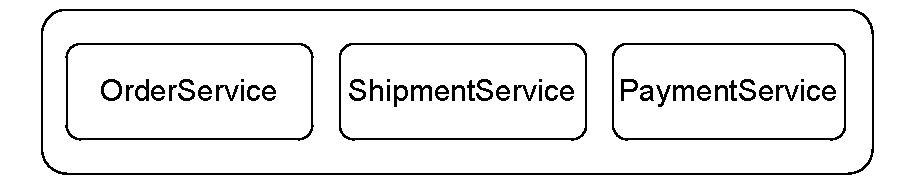
\includegraphics[width=0.4\textwidth]{images/mono/mono.pdf}
    \caption{Monolith Architektur}
    \label{fig:mono}
\end{figure}

Diese Architektur weist für kleinere Anwendungen gewisse Vorteile auf,
wie eine einfache testbarkeit, Logging, Deployment, sowie Debugging.
Zudem eine Datenbanksynchronisation ist nicht notwendig, da die
gesamte Daten in einer Datenbank persistiert werden. \cite[2]{mono4}

Betrachten wir das E-Commerce-Beispiel.
Dafür definieren wir drei Klassen:
\begin{itemize}
    \item \texttt{OrderService}: Klasse, die die Bestellungen verwaltet
    \item \texttt{PaymentService}: Klasse, die die Zahlungen abwickelt
    \item \texttt{ShipmentService}: Klasse, die die Lieferungen initiiert
\end{itemize}

Die Kommunikation zwischen den Klassen erfolgt durch Methodenaufrufe.
Dabei ist die Klasse \texttt{OrderService} die Hauptklasse, die die anderen Klassen
verwendet, um den Bestellungsvorgang durchzuführen.
Vorteilhaft hier ist, dass hier die Kommunikation zwischen den komponenten einfach ist.
Durch die Verwendung von Methodenaufrufen wird die Komplexität reduziert, die mit
Intersystemkommunikationen verbunden ist.

Jedoch, wenn die Code-Basis wächst und komplex wird, treten einige Nachteile auf.
Durch Änderungen in einer Komponente können unerwartete kaskadierende Fehler
auslösen, was die Weiterentwicklung in kleinen autonomen
Teams erschwert und verlangsamt.

Außerdem durch die Verwendung von direkte Methodenaufrufe, entsteht eine enge Kopplung
zwischen den Komponenten.
Änderungen in der Implementierung oder Signatur einer Methode
können zu kaskadierenden Fehlern führen.

Weiterhin ist die Wiederverwendung von Funktionalitäten nicht möglich, da die
Komponenten eng gekoppelt sind.
Das führt zu Duplikation von Code, was
die Änderungen teurer macht, da die Änderungen in mehreren Stellen durchgeführt werden müssen.

Die dadurch erhöhte Komplexität und die schwierige Wartung führen zu längere Iterationen.
Da das Deployment erfolgt nur als Ganzes und die Iterationen länger dauern,
kommt es zu seltenen Auslieferungen von neuen Features.
Ferner ist Horizontale Skalierung auch nicht möglich, da die Anwendung nur als Ganzes
skaliert werden kann.
Insgesamt ist eine gute Einstiegslösung, allerdings nicht für größere Anwendungen geeignet, da
 die Agilität davon stark betroffen wird.

\subsection{Modular Monolith}
Das Hauptproblem der vorherigen Architektur ist die eng gekoppelte Natur der Architektur,
die eine gewisse Komplexität und Unflexibilität mit sich bringt.
Modulare Monolithen sind eine Evolution der Monolithic  Architektur, die die Vorteile
der Monolithic Architecture erben und gleichzeitig die Nachteile der enge Kopplung verringern.

In diese Architektur wird die Code-Basis in mehrere Module geteilt, die jeweils
eine Teil-Funktionalität der Anwendung implementieren.
Die Kommunikation zwischen den Module erfolgt durch klar definierte Interfaces,
wobei die Wiederverwendbarkeit und Austauschbarkeit der Module ermöglicht wird.\cite[11]{modular-mono2}

Die Trennung in Modulen reduziert zudem die Komplexität und fördert eine bessere
 Organization der Code-Basis, was zu einer bessere Wartbarkeit führt.\cite[2]{modular-mono4}

\begin{figure}[h!]
    \centering
    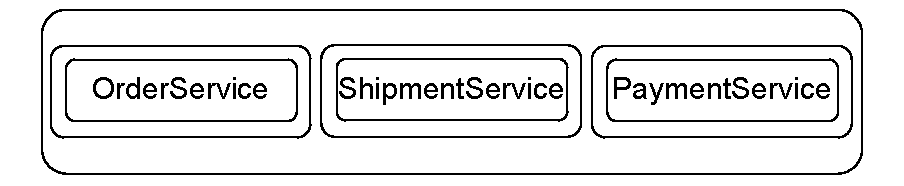
\includegraphics[width=0.4\textwidth]{images/mono/mono-example.pdf}
    \caption{Modular Monolith Architektur}
    \label{fig:modular-mono}
\end{figure}

Betrachten wir erneut das E-Commerce-Beispiel.
Diesmal wird die Anwendung in drei Hauptmodule aufgeteilt:
\begin{itemize}
    \item \texttt{OrderModule}: Verantwortlich für die Verwaltung der Bestellungen
    \item \texttt{PaymentModule}: Verantwortlich für die Abwicklung der Zahlungen
    \item \texttt{ShipmentModule}: Verantwortlich für die Initiierung der Lieferungen
\end{itemize}

Abhängigkeiten zwischen den Modulen werden durch die Verwendungen von Interfaces
reduziert, indem die Module nur die Schnittstellen kennen und nicht die Implementierung.
Zum Beispiel Änderungen an der Implementierung einer Komponente von \texttt{PaymentModule} müssen nur
in der Implementierung des Interfaces durchgeführt werden, ohne dass die anderen
abhängigen Module davon betroffen werden.
Die Modularisierung ermöglicht zusätzlich eine verbesserte Entwicklung in semi-autonomen Teams im
Vergleich zu den traditionellen Monolithen.
Problematisch ist jedoch, dass die Anwendung nur als Ganzes deployt werden kann, was
die Iterationen verlangsamt.
Außerdem ist weiterhin keine horizontale Skalierung möglich und die Funktionalitäten
können nicht wiederverwendet werden, da diese immer noch Teil einer einzigen Anwendung
und eng miteinander gekoppelt sind.

\subsection{Layered}
Das Layered Architektur-Pattern, auch bekannt als n-Tier-Architektur-Pattern, beschreibt eine
Architektur, die die Anwendung in Schichten aufteilt.

Ein wichtige Eigenschaft der Layered Architecture ist der die Trennung der Zuständigkeiten
(Englisch \textit{Separation of concerns}). Komponenten mit unterschiedlichen Aufgaben sollten
auf verschiedene Schichten verteilt werden, sodass die Komponenten einer Schicht jeweils für
eine klar definierte, gemeinsame Aufgabe zuständig sind. \cite[S. 34]{layered2}

Obwohl diese Architektur keine feste Anzahl an Schichten vorschreibt,
bestehen die Layered Architectures meistens aus 3 Schichten~\cite []{layered2}:
\begin{itemize}
\item Presentations-Layer: Verantwortlich für die Interaktion mit dem Benutzer und
die Weiterleitung von Benutzeranfragen an die Business-Layer.
\item Business-Layer: Zuständig für die Verarbeitung von Geschäftslogik und Regeln, die Weiterleitung von Daten zwischen
  die Presentation-Layer und die Data-Layer.
\item Data-Layer: Verantwortlich für die Interaktion mit der Datenbank und die Kommunikation mit der Business-Layer,
um Daten bereitzustellen oder die Ergebnisse entweder an die Presentation-Layer
  oder zurück an den Datenspeicher zu übermitteln.
\end{itemize}

\begin{figure}[h!]
    \centering
    \includegraphics[width=0.3\textwidth]{images/layer.pdf}
    \caption{Layered Architektur}
    \label{fig:layered}
\end{figure}

Ein zentrales Prinzip der Layered Architecture ist der Isolation von Schichten besagt, dass die Kommunikation
zwischen Schichten ausschließlich über definierte Schnittstellen erfolgen sollte.
Dadurch wirken sich Änderungen in einer Schicht nur auf die Schicht selbst sowie höchstens auf eine andere Schicht aus. \cite[10]{layered}

Ein weiteren relevantes Konzept ist die Unterscheidung zwischen offenen und geschlossenen Schichten.
Dieses Konzept beschreibt, wie die Kommunikation zwischen den Schichten organisiert ist.
Standardmäßig sind die Schichten auf Closed gesetzt.
Das bedeutet, dass Module eine Schicht nur die Dienste der direkt darunterliegenden Schicht nutzen können.
\cite{layered}[S. 3].(Siehe Abb. ~\ref{fig:layered-request-flow})

Diese Struktur fördert die Isolation von Schichten und reduziert somit die Abhängigkeiten zwischen den Schichten, da
 Schichten nur Abhängigkeiten zu den direkt darunterliegenden Schichten haben und nicht zu Schichten, die oberhalb liegen.
Dadurch werden zyklischen Abhängigkeiten zwischen Schichten vermieden, was Änderungen in einer Schicht erleichtert.

Im Gegensatz dazu erlauben offene Schichten den Zugriff auf die Funktionalitäten von Schichten, die beliebig
weit entfernt sind und nicht nur auf die Funktionalitäten der unmittelbaren darunterliegenden Schicht.
(Siehe Abb. ~\ref{fig:layered-request-flow}). \cite[4]{layered}

Das kann besonders nützlich sein, wenn z.B. Anfragen kein Mehrwert durch das
Durchlaufen eine bestimmte Schicht bwz. Schichten erhalten und nur weitergeleitet werden.
Dieses Phänomen wird auch als \texttt{sinkhole anti-pattern} bezeichnet und das kann durch die
Verwendung von offene Schichten vermieden werden.

Einerseits reduziert die Nutzung von offenen Schichten die unnötigen Aufwand für die Logik der Weiterleitung von Anfragen,
 andererseits verletzt das das Prinzip der Isolation von Schichten.
Folglich Änderungen in einer Schicht können sich auf mehrere Schichten auswirken, was die Flexibilität und Wartbarkeit
des Systems beeinträchtigt.[7 - 8]\cite{layered}

\begin{figure}[h!]
    \centering
    \includegraphics[width=0.3\textwidth]{images/layer2.pdf}
    \caption{Open/Close Layering}
    \label{fig:layered-request-flow}
\end{figure}

Die Implementierung dieser Architektur bietet eine Reihe von Vorteilen.
Durch die Aufteilung des Systems in verschiedene Schichten wird eine unabhängige
Entwicklung und Wartung der einzelnen Schichten ermöglicht ~\cite{layered2}[S. 35].
Ein weiterer Vorteil besteht darin, dass der Zugriff auf die Dienste zwischen den
Schichten über Schnittstellen (Interfaces) erfolgt.
Dadurch sind Entwickler nicht gezwungen, die interne Implementierung einer Schicht zu kennen, um die bereitgestellten
Dienste nutzen zu können. \cite{layered4}[S. 11]
Aufgrund der losen Kopplung der Schichten ist es zudem möglich, neue Funktionalitäten
hinzuzufügen durch die Einführung neuer Schichten ohne dabei umfangreiche Anpassungen am gesamten
System vornehmen zu müssen \cite{layered2}[S. 35].
Allerdings führt die Nutzung dieser Architektur zu einer geringeren Performance, da für
den Zugriff auf Dienste in unteren Schichten eine Kette von Anfrageweiterleitungen erforderlich ist ~\cite{layered4}[S. 11].
\section{Moderne Enterprise-Architekturen}

\subsection{Event-Driven Architecture}
Die Event-Driven Architecture wählt als Basis einen anderen Ausgangspunkt als die bisherigen Architekturmuster.
Während bei letzteren Komponenten Dienste bereitstellen, welche von anderen Komponenten explizit genutzt werden,
verhalten sich Dienst-bereitstellende Komponenten in der Event-Driven Architecture reaktiv,
werden also implizit von Dienst-konsumierenden Komponenten genutzt \cite{garlanShawImplizit}.
Ein System reagiert somit asynchron auf Zustandsänderungen, also Ereignisse in diesem System \cite{eda}.
Die in dieser Architektur minimalen Einheiten, welche Informationen einer Zustandsänderung kapseln, werden \textit{Events} genannt.
Die Idee der impliziten Behandlung von Ereignissen ist nicht neu und taucht erstmals 1994 im von Garlan und Shaw publizierten Papier
\textit{\enquote{An introduction to Software Architecture}} auf.

Betrachten wir im Folgenden die Basis-Bestandteile der Event-Driven Architecture:
\begin{itemize}
  \item Ereignis (englisch \textit{Event}): Kapselt Information einer Zustandsänderung eines Systems
  \item Produzent (englisch \textit{Producer}): Komponente, die Event erzeugt
  \item Herausgeber (englisch \textit{Publisher}): Komponente, die, von Produzenten erzeugte, Events publiziert
  \item Konsument (englisch \textit{Consumer}): Reagiert auf publizierte Events
  \item Vermittler (englisch \textit{Mediator}): Liegt zwischen Produzenten und Konsumenten - filtert Events und verteilt diese auf Konsumenten
  \item Event-Bus: Oft auch \textit{Event-Broker} genannt - bietet die Infrastruktur für die Gesamtheit der Vermittler
\end{itemize}
Abstrakt kann ein Event als ein Vertrag zwischen Produzenten und Konsumenten am Event-Bus betrachtet werden.
Der Konsument nutzt die Spezifikation des Events am Bus, der Produzent implementiert jene Spezifikation.
Abbildung \ref{fig:eda} stellt diesen Vertrag dar.

\begin{figure}[!h]
  \centering
  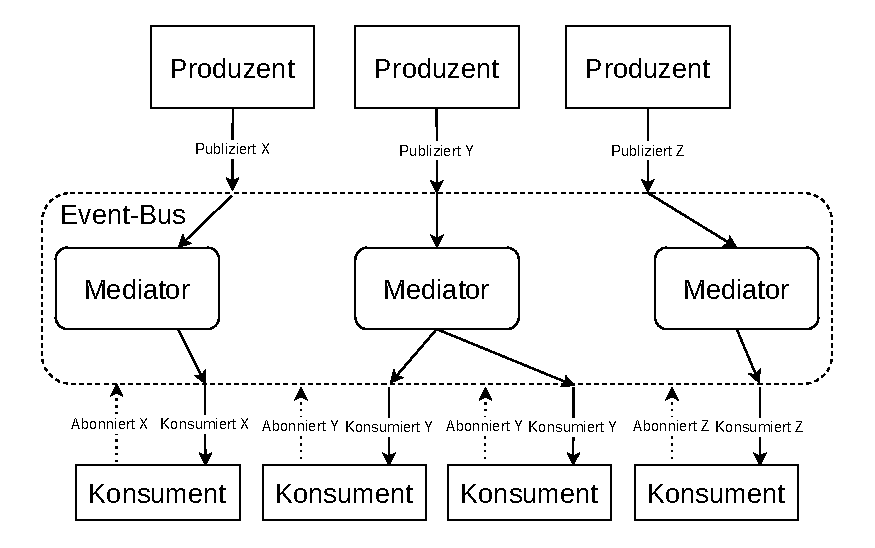
\includegraphics[width=\linewidth]{images/eda/eda.drawio}
  \caption{Vertrag zwischen Produzenten und Konsumenten am Event-Bus}
  \label{fig:eda}
\end{figure}

Durch den Vertrag weisen die Events am Event-Bus starke Kohäsion und somit lose Kopplung auf.
Diese lose Kopplung minimiert nicht nur kaskadierende Fehler, sondern ermöglicht agilen Entwickler-Teams durch klar abgegrenzte Features einfach definierbare Iterationen
- eine Menge von Events, deren Erzeugung und Konsumierung.

Weiter sind Events oft nah an dem, was Ereignisse in realen Prozessen sind, also domain-driven.
Gebündelt ermöglichen obige Punkte die kontinuierliche Auslieferung von Software in kurzen Intervallen.

Außerdem garantiert die asynchrone Behandlung von Ereignissen zusammen mit der loosen Kopplung maximale Skalierung.
Daher sind Event-Driven Architekturen besonders für datenintensive Echtzeit-Anwendungen wie IoT (Internet of Things) und Analytics geeignet \cite{iotEda}.

Die Agilität der Architektur kann weiter erhöht werden, indem der event-basierte Aspekt mit weiteren agilen Strukturen wie Microservices oder cloud-nativen Serverless-Functions kombiniert wird.
Die damit einhergehende Komplexität stellt teilweise hohe Anforderungen an die Entwickler.
Aufgrund der Asynchronität der Behandlung von Ereignissen ist die Testung des Systems meist schwer und die Fehlerbehandlung essentiell.
Mögliche Problemquellen schließen dabei unter anderem Event-Verlust, erhöhte Latenz und Inkonsistenz ein.
Die hohen Anforderungen an die Entwickler verlangen viel Vertrauen in jene, einer der zentralen Punkte des agilen Manifests \cite{agileManifesto}.
Insgesamt weist die Event-Driven Architecture also eine sehr hohe Agilität auf und ist damit besonders für moderne Software und ihre stetig wechselnden Anforderungen geeignet.

% TODO: Jetzt bestenfalls übergreifendes Beispiel

\section{Fallstudien und Praxisbeispiele}
Blah \ldots

\section{Diskussion}

\section{Zusammenfassung und Ausblick}
%(Überblick über die gesamte Arbeit, Rückführung auf Aussagen aus Kapitel 1 durchführen, offene Punkte als neue Forschungsfragen definieren)






\bibliographystyle{ACM-Reference-Format}
\bibliography{main}

\appendix

\section{Anhang 1}

\subsection{Übungsaufgaben}
Blah \ldots

\section{Anhang 2}
Blah \ldots

\end{document}
\endinput
